\documentclass[]{jsarticle}
\usepackage[dvipdfmx]{graphicx}

\title{体育学年末レポート}
\author{Ec3 32 平田蓮}
\date{}

\begin{document}
\maketitle
\section{はじめに}
日本語を母語とする人ならば、誰しもが敬語というものに馴染みがあるはずである。
頭が良いクラスメイトも、人気の俳優も、総理大臣も、もちろんオリンピック選手も。
人々から一目置かれている彼ら、彼女らも、また一目置いている私たちも
日常的に敬語を使うからである。私たち一般人が届かないと思っているような
彼らにも私たちと同じような一面がある。中学生の頃、同級生に2020年東京オリンピック
の代表候補とまでいわれていた体操選手がいた。しかし、今彼女が何をしているか私は知らないし、
おそらく私が彼女の情報を探して実際に東京オリンピック開催時にTV放送をみることもない。
私と、おそらく中学校にいた友人たちの間では、彼女は「オリンピック選手」ではなく、
他の人たちと何ら変わりない「友人」のひとりに過ぎなかったからだ。

現代のオリンピック選手は、いわゆる「スター」の一面を持っている。
昨年はじめに引退を発表したレスリングの吉田沙保里選手、
数々の平泳ぎの世界記録や日本記録を打ち立てている競泳の北島康介選手など、
彼らは数多くの人の注目を集め、憧れを持つ人も少なくない。
時として「スター」になって世界で活躍する彼らも、
オフシーズンは会社員であったり、いわゆる我々一般人と変わりないのである。
そんなオリンピック選手に注目しながら今までのオリンピックの歴史を振り返りつつ、
学年末レポートとする。

\section{オリンピック選手という存在}
まず、現代のオリンピック(以下: 近代オリンピック)の起源であるオリンピア祭典競技、
いわゆる古代オリンピックについて触れる。
正確ではないが、古代オリンピックが始まったのは紀元前9世紀頃であると考えられている。
近代オリンピックはスポーツの祭典であるが、
オリンピア祭典競技は神々を崇める宗教行事であった。
その頃のオリンピック選手は、文字通り「英雄」として讃えられた。
神々を崇める行事に参加した英雄で、実際に一般人とは一線を画す存在であった。
彼らは、時として一般人と同じである現在のオリンピック選手よりもさらに非一般的な神に近い存在
であったのだ。
しかし、この頃は女子禁制の行事で、選手は全員男子であった。
現在のように女子選手が登場したのは近代オリンピックになってからである。

近代オリンピックが始まったのは1896年である。
しかし、第一回のアテネ大会ではまだ男子のみの選手が参加した。
参加選手数は200人強と、2016年のリオデジャネイロオリンピックの11000人
には遠く及ばない人数である。
当時は、世界的な大会としてではなく、ヨーロッパの先進国同士が集まって開催をしたので、
参加国も少なく、規模はとても少ないものであった。
選手の知名度も現在とは打って変わり、
古代オリンピックとは真逆に、普通の一般人と変わる点は少なかった。

\section{悲惨な事件}
近代オリンピックはその後も徐々にその知名度を上げ、
今の知名度を誇るに至った。
オリンピック選手という存在を世に広める大きな事件の一つに、
1972年ミュンヘンオリンピックで起きた「黒い九月事件」がある。
パレスチナの武装組織「黒い九月」がイスラエルのオリンピック選手たちを殺害したテロ事件である。
オリンピック開催中の期間に、8人のテロリストが選手村に侵入し、
2人を殺害したのち、9人を人質に取った。
最終的に、人質を乗せたヘリコプターが爆破し、全員が死亡してしまうという最悪の結末で事件は完結した。
この事件で11人のオリンピック選手が犠牲となり、
世界に悲痛な記憶を刻み付けた。

この事件が起きた背景には、杜撰な選手村の警備体制があったという。
当時は今ほど厳重な警備が敷かれておらず、
この大会以降の警備強化につながった。
また、この事件を通してオリンピック選手というものが世界により一層広まった。

\begin{figure}[h]
    \centering
    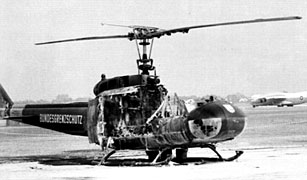
\includegraphics{heli.jpg}
    \caption{テロで爆破されたヘリコプター}
\end{figure}

\section{2020東京オリンピックで期待されること}
さて、世界情勢というものはいつも不安定で、
つい先月も「第三次世界大戦」という不吉なワードが人々の間で交わされた。
こんな世の中で約半年後に行われる東京オリンピックでは最強レベルの警備体制が敷かれることであろう。
幸い、第20回ミュンヘンオリンピック以降、このような悲惨な事件は起きていないので、
今大会も何事もなくすぎるように願うばかりである。

100年以上前、夢にすら思われていなかった100m走の10秒切りを
1968年にアメリカのシム・ハインズ選手が破ったように、
スポーツのアスリート選手には無限の可能性が秘められている。
今後も100年、200年とオリンピックやその他のスポーツ競技大会が続くことを願う。
そのためには、過去の凄惨な事件から得た教訓を忘れないことが大切である。

日本の技術力は世界クラスの評価を受けている。
1964年の東京オリンピックでは、新幹線やカラーテレビなど、当時の日本の最新技術が世界中に注目された。
これは単に日本の技術力が高いだけでなく、
日本人の丁寧な人間性などが評価されていた。
今回の東京オリンピックでも、日本人の丁寧な仕事でテロなどの警備を行うことが期待されている。
また、我々もこの技術力を担うエンジニアの卵として、
関心を持ち、常に新しい情報を求めてこの情報社会を生き抜いていくべきである。

\section{これからのオリンピック}
ここまで、過去にあった悲惨な事件について触れながら、オリンピック選手という存在について書いてきた。
これからの技術の発展に伴い、過去にあったような選手を巻き込む事件はなくなると考えられる。
ではこの先、選手に降りかかる火の粉はないであろうか。
否、人的要因が関わらない危険なども考えられる。

身近な例としては熱中症が挙げられる。
年々「地球温暖化」と謳われ続けているように世界の平均気温が上昇しつつある。
実際に、長岡の平均降雪量も低下を辿る一方である。
この地球温暖化のせいで、特にスポーツ選手が死に至る最悪のケースも
年々増えている。
また、熱中症に関しては選手だけではなく、観戦客も注意をする必要がある。
東京オリンピックではもちろんのこと、今後のオリンピックでも会場などでの熱中症対策が重要になってくることは
間違いない。

地球温暖化は排気ガスなどによる温室効果が原因だであると言われている。
図\ref{fig:graph}にグラフを示す。
このグラフを見てもわかるように、
人間の技術力の進歩に伴って地球上の二酸化炭素濃度は増加を続けている。

\begin{figure}[h]
    \centering
    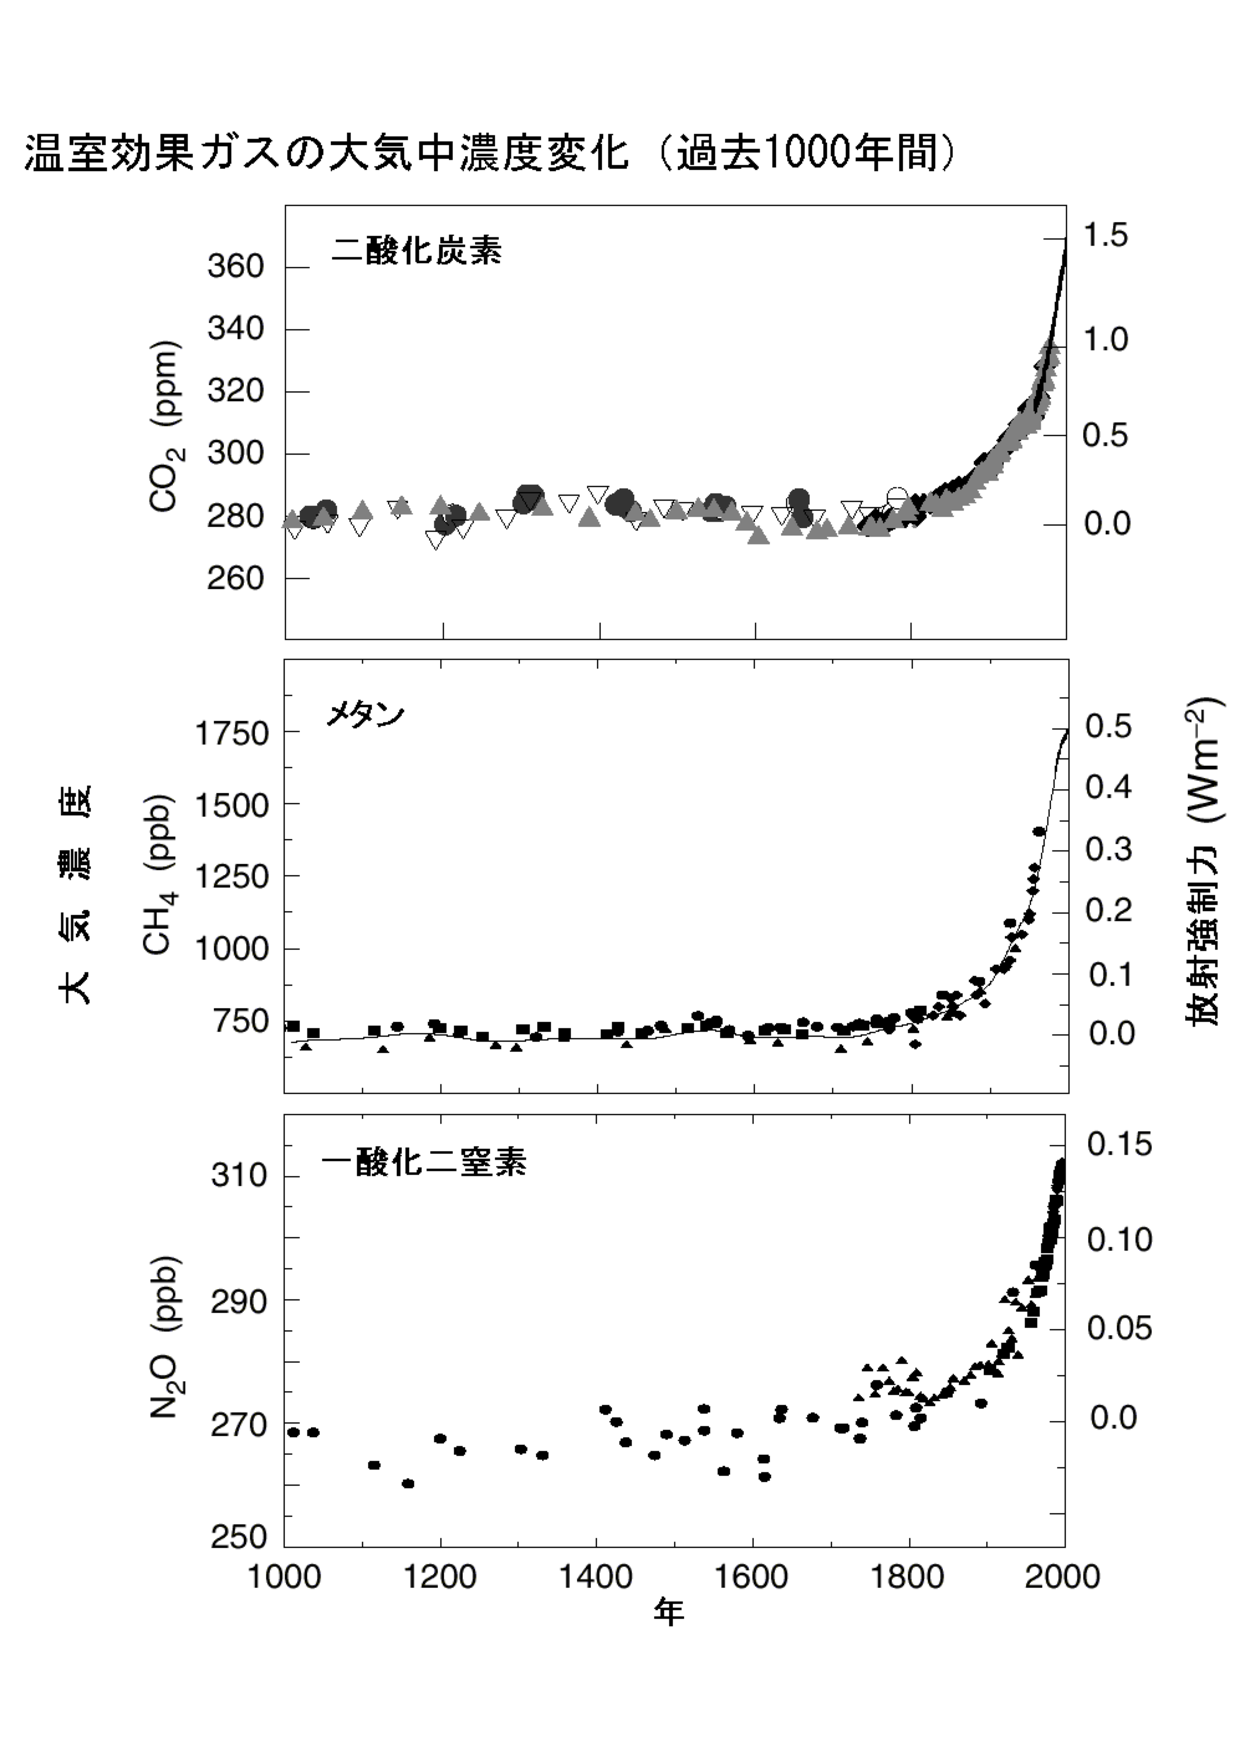
\includegraphics[width=9cm]{graph.pdf}
    \caption{地球の空気中の二酸化炭素濃度の変化}
    \label{fig:graph}
\end{figure}

このことから、技術力の上昇と熱中症のリスクはトレードオフの関係にあることがわかる。
我々技術者の卵は、ただただ今ある技術を発展させていくだけでなく、
地球環境と共存していくことを考えなければならない。

さて、現代を生きる我々に数百万、数千万年後の地球を考えることはできるだろうか。

\begin{thebibliography}{99}
    \bibitem{history} オリンピックの歴史 日本オリンピック委員会 \\
        https://www.joc.or.jp/sp/column/olympic/history/001.html
        (閲覧日: 2020/2/15)
    \bibitem{munhen} そのとき時代が変わった NewsDigest \\
        http://www.newsdigest.de/newsde/column/jidai/2352-muenchner-olympia-attentat/ \\
        (閲覧日: 2020/2/15)
    \bibitem{hot} 地球温暖化の原因と予測 全国地球温暖化予防活動推進センター \\
        https://www.jccca.org/global\_warming/knowledge/kno02.html
        (閲覧日: 2020/2/24)
    \bibitem{hot2} ミランコビッチ・サイクルの今日的な意義 インブリー著「氷河時代の謎をとく」(1979年)を読み直して \\
        http://fnorio.com/0188Imbrie\_1979/Imbrie\_1979.html
        (閲覧日: 2020/2/24)
\end{thebibliography}
\end{document}